As said before the translation cache can have multiple implementations, one of them is using a hash table format to manage the storage of more than one basic block. 

\begin{figure} [h!]
	\centering
	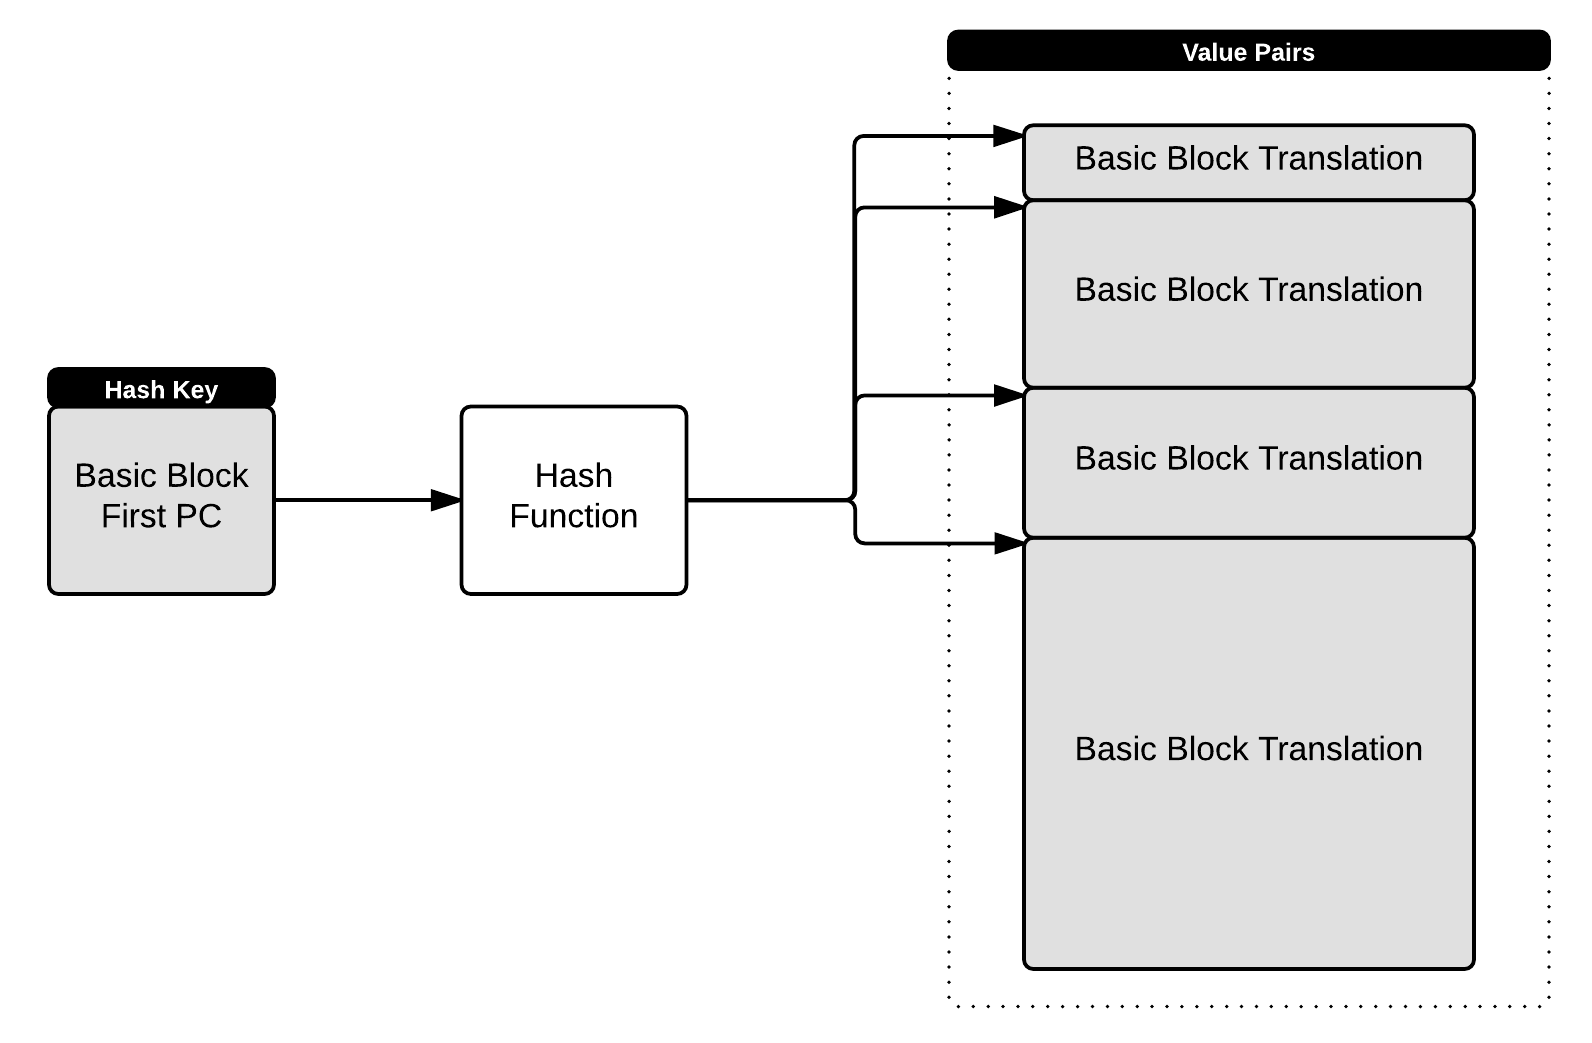
\includegraphics[scale = 0.2]{images/Hash.png}
	\caption{Mechanism for the hash table management.}
	\label{fig:Hash}
\end{figure}

This implementation has to respect the translation cache interface and so the following functions need to be implemented:
\begin{itemize}
	\item addtag - adds a new element to the list of basic blocks. We need to save the initial PC of the basic block that is passed as argument, the starting address of the basic block in the translation cache is equal to the address of the previous basic block plus the size of the previous basic block, and the size of the new basic block is set to zero.
	\item gettransaddr - this function receives a PC and compares it to the initial PC from each element in the basic block list and if there is a hit, the starting address of the corresponding basic block is returned.
	\item cachecode - this function is used to write in the translation cache. Two function need to be implemented, one to write one word, and one to write two words in the translation cache. To perform a write operation, we first need to check if there is enough room left for what we want to write. If there isn't, it is necessary to remove the oldest basic block in cache. But, even if there is room in the cache, another verification is needed. It's necessary to check if the basic block address plus the basic block size plus the new code size is bigger than the memory size. This means that we are in the end of the translation cache and the space that is available is in the beginning of the cache. When this happens we need to copy the basic block to the memory beginning and only then perform the write operation. To do this it's necessary to make room in the memory beginning to copy the entire basic block.
\end{itemize}
